%Summary: Introduce idea of end to end toolflow
%Goal: Defend the idea that we can design an instrument using only a simple high level specification

%Summary: describe CASPER, PASP and reconfigurable heterogeneous setispec Goals:
%describe the existence and continued development of �blocks�
%show the ability to design reconfigurable instruments by adding a layer of abstraction to the CASPER+xgpu work


%TODO: explicitly discuss implementation, code, package, where to get it, etc

\chapter{High Level Toolflow}
\label{chap:High Level Toolflow}


Instrument design is often done by building the instrument from scratch.
This work extends the CASPER philosophy, demonstrating that entire heterogeneous instruments can be designed with minimal user input.
Rather than designing a completely different instrument for every different specification, this software package is parameterized so a changes can  %TODO: change this - only requires a recompile.

%TODO
In this chapter, I introduce a toolflow I developed called ORCAS or Optimal Rearrangement of Cluster-based Astronomy Signal processing.

Introduction - resummarize problem solved by this work
overview of the steps in the process



%A number of options are available but which is best?
%Need to understand how to choose the right platform(s) for each implementation
%With constant changes in technology and algorithm implementations an automatic approach is required



%Describe what the tool flow should to, for whom, etc
\section{ORCAS Goals} \label{High Level Toolflow:ORCAS Goals}
ORCAS extends the CASPER philosophy discussed in Section \ref{Related Work:Radio Astronomy} by providing an end-to-end toolflow that allows the user to go from a high level description of the instrument to a low level mapping automatically. 
While the CASPER toolflow has proven successful in the FPGA domain, it's not always clear that FPGAs are the most cost-effective implementation for a given instrument.
The ORCAS captures the successful elements of the CASPER tools while extending its reach to the heterogeneous domain. 
One of the most important elements of the CASPER tools is the library of DSP blocks. 
The CASPER library blocks are constantly being updated, ensuring that the library can always be compiled on the latest technology.
By incorporating existing libraries implemented for CPUs, such as FFTW,  of GPUs, like cuBLAS, xGPU, and CUFFT, ORCAS can also keep up with changing technology, without the need for constant updates to the tool itself.
The flexibility of the libraries also allows us to buy technology at the last minute, ensuring we get the cheapest price available for an instrument that will provide the needed performance.

In addition to the elements drawn from the CASPER library, ORCAS emphasizes a twofold approach to cost reduction in instrument design.
The first cost savings is in the design time.
The tool is designed to map designs to hardware within a few hours. 
This fast mapping makes it possible to quickly assess performance on new or nonexistent technology and allows the designer to assess the impact of potential optimizations, making it easy to test a number of different design ideas without spending time testing different implementations.
By incorporating tested libraries, there is much less debugging needed in the eventual implementations.


The second cost ORCAS is able to reduce is the cost of the instrument itself.
While the implementation of a design has been greatly simplified by the availability of tools described in Section \ref{Related Work:Radio Astronomy}, none of those tools help determine which type of hardware is best. 
The extensive library allows the tool to support whatever hardware is cheapest, allowing the choice of hardware to be completely determined based on cost.
This cost could be defined in a number of ways, depending on which parameters the instrument designer needs to minimize. 
Obviously the cost could refer to the monetary price of the hardware, but the tool can also be used to minimize the amount of power needed by the instrument, the physical size of the instrument, and other user defined costs.


%Goals
%Interface
%Accessible to astronomers (domain experts)
ORCAS is designed to be be accessible to both computer experts and radio astronomers, or other domain experts.
For a domain expert,  ORCAS allows the user to choose a predefined instrument type and select high level parameters without worrying how it will ultimately map to hardware. 
%Accessible computer experts
%Implementation
%Generate code for an instrument optimally mapped across a heterogeneous cluster
%Retain improvements offered by low-level optimization

The computer expert can use the tool to define a new instrument, by specifying the algorithm, and is able to provide optimization.
%TODO: fix this, I don't like it
For example, if an engineer wrote an optimized FFT algorithm, the tool will be able to incorporate that into the final optimized result.
In the end, regardless of who is using this tool, a cost-optimal mapping of the instrument gets produced. 

\begin{figure}[ht!]
  \centering
    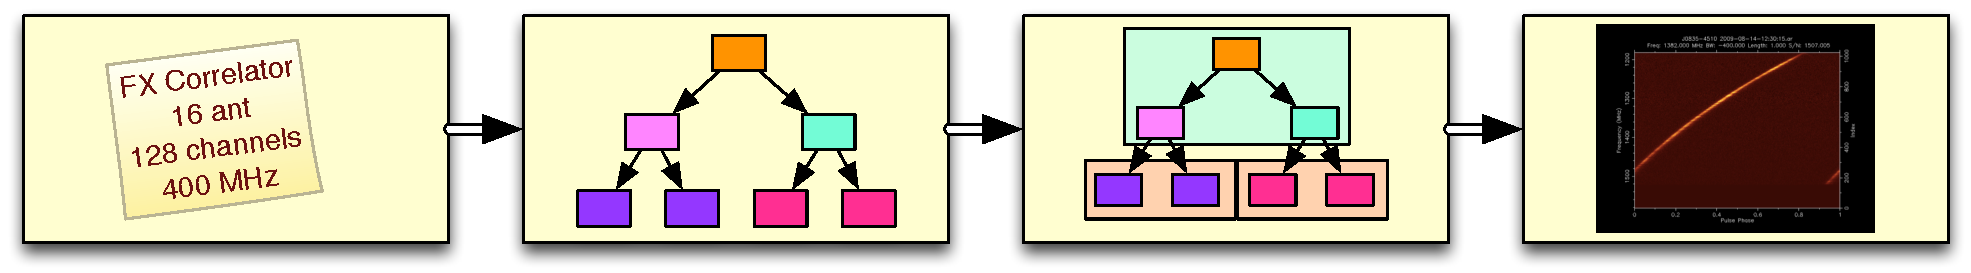
\includegraphics[width=1\textwidth]{Images/C4/toolflow_horizontal.pdf}
  \caption{The Four Stage ORCAS Toolflow}
  \label{fig: C4/toolflow_horizontal.pdf}
\end{figure}

These goals are achieved through a four stage tool that allows the user to go from a high level description of an instrument to an optimized cluster design. 
Each stage of the ORCAS toolflow is represented in Figure \ref{fig: C4/toolflow_horizontal.pdf}. 
The first stage is instrument definition, which is described in Section \ref{High Level Toolflow:Instrument Definition}. 
This stage is designed to fit the needs of the domain expert. 
It allows the radio astronomer to create a predefined instrument using a handful of parameters. 
The instrument definition is converted into a dataflow model, as described in Section \ref{High Level Toolflow:Dataflow Model}. 
The second stage, the dataflow model, is aimed at the computer expect, since it allows for a more detailed and flexible definition of the algorithm than the previous stage and provides the means to include optimized blocks.  
The dataflow model represents an abstract definition of the algorithm without taking into account the eventual hardware target. 
The next stage, appropriately named mapping, maps the dataflow model to specific hardware. 
In the mapping stage, each block defined by the dataflow model gets mapped to a specific piece of hardware. 
This stage takes into account hardware and network limitations to produce a cost optimal mapping of the original dataflow. 
Mapping is discussed in Section \ref{High Level Toolflow:Mapping} and Chapter \ref{chap:Algorithm Partitioning} provides more details about the algorithm used to produce a mapped instrument and the performance of that algorithm.
Finally, once each block has been mapped to a piece of hardware, the code can be stitched together into a working instrument, as presented in Section \ref{High Level Toolflow:Code Generation}. 
The rest of the chapter will describe each stage of the toolflow in more detail and explain how they are designed to meet the needs of the users they are targeting.



\section{Instrument Definition} \label{High Level Toolflow:Instrument Definition}

\begin{figure}[ht!]
  \centering
    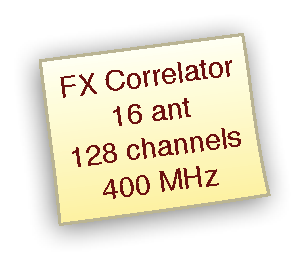
\includegraphics[width=0.5\textwidth]{Images/C4/instrument_description.pdf}
  \caption{ORCAS Toolflow Instrument Definition}
  \label{fig: C4/instrument_description.pdf}
\end{figure}

In the first step in the ORCAS toolflow, the user must describe the instrument using high level parameters. 
These parameters should all be relevant to the astronomer and abstract away any implementation details that do not pertain to the scientific goals. 
While it would be easy to expose many of the low level parameters at this top layer, this would force the domain expert to become a computer expert as well, exactly the scenario this tool is aiming to avoid. 


The instrument description as represented in Figure \ref{fig: C4/instrument_description.pdf} fits on a small sticky note. 
The idea that the parameters should be so few that they fit on a single sticky note was the driving force behind the instrument definition. 
An instrument designer who finds that he or she needs additional control beyond what is provided by the instrument description always has the flexibility to work with the dataflow model directly, where many low level parameters are exposed. 
Additional instruments or new parameters for existing instruments can be added by defining how those parameters affect the final dataflow diagram. 

%TODO: exploration
%TODO: discuss this more thoroughly
\subsection{Design space exploration}
In addition to defining a single instrument, an astronomer can use this tool to explore different implementations and assess the tradeoff in cost vs additional processing. 
Rather than specifying single values for the instrument parameters, the astronomer can choose a range to search through and have it generate a design, and an associated cost, for each value. 
This proves valuable when the specification of an instrument isn't fully defined.
In the case of a high resolution spectrometer, the astronomer could adjust the number of coarse and fine channels, keeping the spectral resolution the same, to find the cheapest design that achieves that resolution.
For polyphase filter banks, the number of taps in the FIR can be varied to assess the increase in cost associated with a better filter response.
Even non-numerical parameters can be varied, such as the FIR window type, to see how it will affect the eventual design.





%TODO: add filter parameters, ntaps, window (?)




%Describe instrument using parameters an astronomer can understand
%Small number of predefined instrument types
%Need to input
%Instrument type (predefined patterns)
%Total Bandwidth
%Array size (n)
%Etc
%Generates a dataflow representation










\section{Dataflow Model} \label{High Level Toolflow:Dataflow Model}
%TODO: Add tool name
\begin{figure}[ht!]
  \centering
    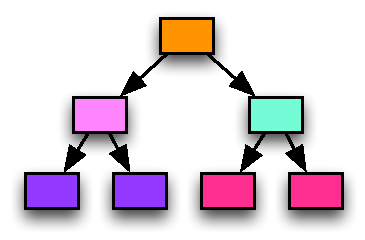
\includegraphics[width=0.75\textwidth]{Images/C4/dataflow_model.pdf}
  \caption{The ORCAS Toolflow: Dataflow Model}
  \label{fig: C4/dataflow_model.pdf}
\end{figure}

The second step of the toolflow translates the instrument definition into a dataflow model. 
%Dataflow representation of instrument
%Define input/output connections
%Define input/output bandwidth
%Generates a series of blocks configured to talk to each other

\subsection{Computational Blocks}
Building blocks
%Collection of blocks necessary to solve most problems
%Can be parameterized
%Include a method to assess performance on each (supported) platform
%Performance model
%Benchmark
%Unit tests
%Uniform interconnect model
%Optimization: remove interconnect overhead for cores running on the same hardware



%Optimization already exists
\cite{Govindaraju:2008vx} %replace with more recent fft alt
\cite{Kestur:2010tn}


\subsection{Connection Types}
%TODO: edit this a lot
Suppose we know we have 2 types of blocks: $A$, and $B$ and blocks of type $A$ must send their data to blocks of type $B$.
We need to definite the communication patterns between $A$ blocks and $B$ blocks.
This could happen in 2 ways, `one-to-one' and `all-to-all'. 

%TODO: fix references
\begin{figure}
  \centering
    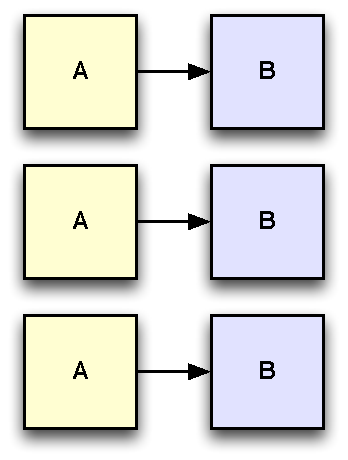
\includegraphics[height=0.43\textheight]{Images/C5/one-to-one.pdf}
    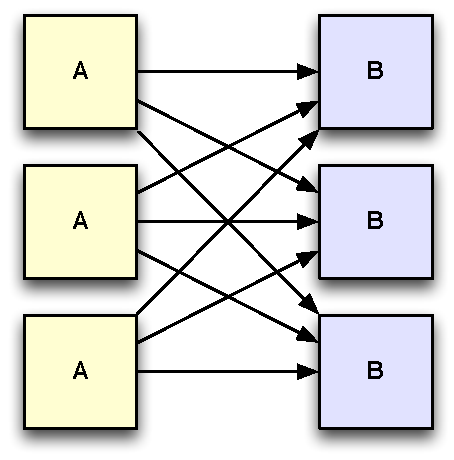
\includegraphics[height=0.43\textheight]{Images/C5/all-to-all.pdf}
  \caption{TODO}
  \label{fig:C4/one-to-one.pdf}
\end{figure}

A `one-to-one' connection is where every $A$ block communicates with exactly one $B$ block, as shown in Figure \ref{fig:C4/one-to-one.pdf}. 
With this type of connection, the number of $A$ blocks must be equal to the number of $B$ blocks.
The F-engines in a FX correlator are a good example of this type of connection. 
The correlator has an F-engine for each antenna, each containing the same blocks linked in the same way. 
Within an F-engine, a PFB\_FIR filter must communicate with a single FFT.
In general, every PFB\_FIR within an F-engine, blocktype `A' must communicate with exactly one FFT, blocktype `B'. 

An `all-to-all' connection occurs when every $A$ block must send some data to ever $B$ block. 
Figure \ref{fig:C4/one-to-one.pdf} shows what an all-to-all connection between three $A$ blocks and three $B$ blocks will look like. 
In this case, every $A$ block must send some data to every $B$ block. 
For example, the type of connection between the per-antenna FFTs and the per-channel X-engines in an FX correlator would be `all-to-all'. 
Each X-engine needs a small amount of data from every F-engine to compute the cross-correlations from a single channel. 
In the `all-to-all' case, there is no reason for the number of sending nodes needs to be the same as the number of receiving nodes. 
%The n's do not get introduced until the ILP is defined
%This means that $n_{i,A}$ and $n_{i,B}$ do not have to be equal, and as long as the data can be distributed appropriately, there is no enforced relationship between the two variables. 




\begin{figure}
  \centering
    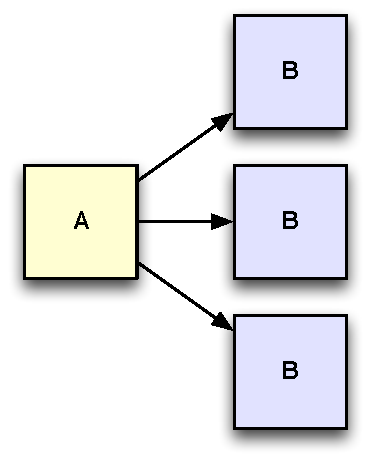
\includegraphics[height=0.45\textheight]{Images/C5/one-to-all.pdf}
    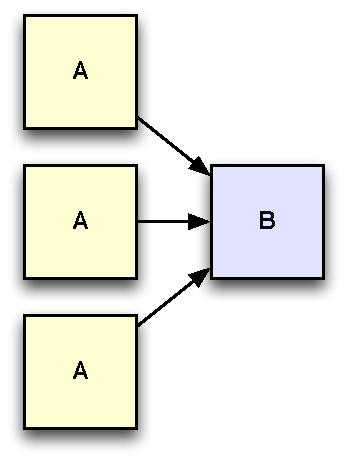
\includegraphics[height=0.45\textheight]{Images/C5/all-to-one.pdf}
  \caption{TODO}
  \label{fig: C4/one-to-all_vs_all-to-one}
\end{figure}



It might seem like there are two more possible types of connection that need to be defined, `one-to-all' and `all-to-one' .
A data flow with a `one-to-all' connection, shown on the left in Figure \ref{fig: C4/one-to-all_vs_all-to-one} would have exactly one $A$ block that needs to send data to many $B$ blocks. 
This is exemplified in the dataflow for a high-resolution spectrometer.
The coarse channelization is done in a single FFT block, which then needs to send the data to many other FFTs to do the fine channelization. 
The `all-to-one' connection is also shown on the right in Figure \ref{fig: C4/one-to-all_vs_all-to-one}
is the reverse of the `one-to-all' case. 
In this type of connection, there are many $A$ blocks and they all need to send data to a single instance of a $B$ block. 
An example of this arises when some processing is done in a distributed manner but the instrument needs to record the final result in a central place. 

It turns out, these are both special instances of the `all-to-all' connection. 
The `one-to-all' connection is simply an `all-to-all' where the number of $A$ blocks is fixed at one.
Similarly, the `all-to-one' connection is also an `all-to-all' where the number of $B$ blocks is fixed at one.
Because of this, there is no need to include or support these cases as unique connection types. 


While it may seem like additional link types exist like `all-to-some' or `one-to-some', this turns out to be impossible. 
Either a block of type $A$ cannot send its data to only some blocks of type $B$ because of the way blocktypes are defined.
Any block of the same type should be interchangeable with another block of the same type.
In an `all-to-some' connection, blocks of type $A$ would need to send data to $B_1$ but not send data to $B_2$.
But that connection patterns implies that the blocks $B_1$ and $B_2$ are \emph{not} interchangeable and therefore cannot have the same blocktype.


%TODO: This isn't implemented in the ILP
%TODO: Add correlator beamformer example. 
%This does not preclude asymmetrical designs. 
%Instead, asymmetry is supported by allowing blocks to define a list of blocktypes they must send data to or receive data from. 
%The connection between any two blocktypes still must be described as above.

%\subsection{Translating Instrument Definitions to Dataflow Diagrams}
% Describe data flow for each instrument we are interested in implementing
%Now that we have a method for describing a general dataflow, we will describe how each type of instrument definition described in the previous section is converted to a dataflow. 
%Multiple antennas?






\section{Mapping}  \label{High Level Toolflow:Mapping}
%TODO: Add tool name
%\begin{figure}[h!]
%  \centering
%    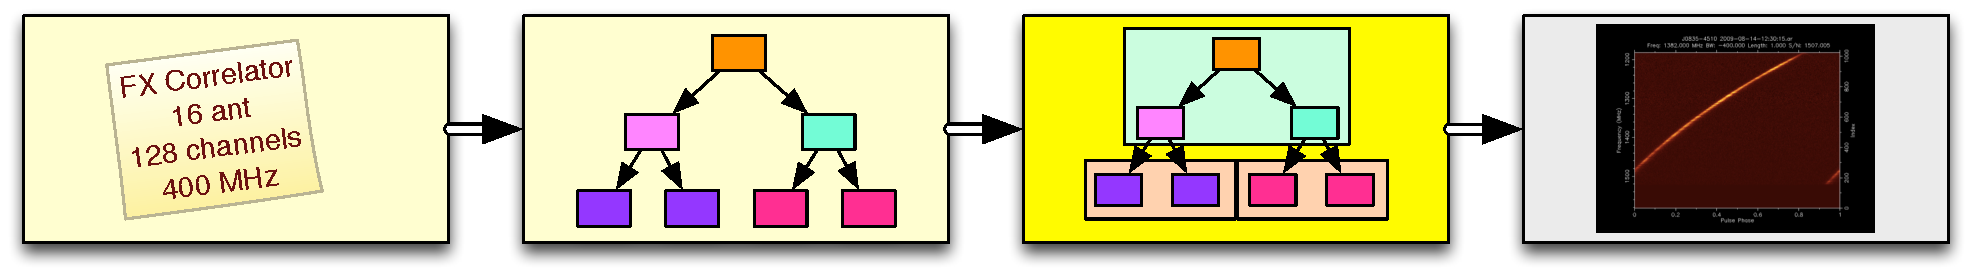
\includegraphics[width=1\textwidth]{Images/C4/toolflow_horizontal_s3.pdf}
%  \caption{ORCAS Toolflow: Mapping}
%  \label{fig: C4/toolflow_horizontal_s3.pdf}
%\end{figure}

\begin{figure}[ht!]
  \centering
    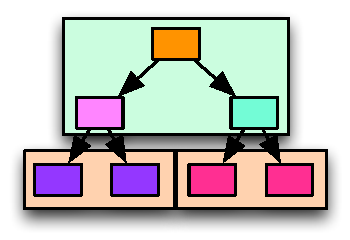
\includegraphics[width=0.75\textwidth]{Images/C4/mapped_dataflow.pdf}
  \caption{The ORCAS Toolflow: Mapped Dataflow Representation}
  \label{fig: C4/mapped_dataflow.pdf}
\end{figure}

Once the dataflow and the computational blocks are defined, ORCAS must determine how to place each computational block into hardware. 
In the mapping stage, ORCAS determines what type of hardware should be used for each block, while minimizing the total cost of the hardware (in dollars, watts, or another used-defined metric).
The icon in Figure \ref{fig: C4/mapped_dataflow.pdf} represents the mapping phase of the toolflow. 

%Not certain this belongs here, possibly should go with the models?
%Before mapping, need to determine which blocks can be mapped to which platforms
%Synthesize/compile existing implementations to determine which platforms can support the spec
%Sanity check bandwidth requirements
%Test for acceptable noise tolerance in different implementations
%Known signals
%Test against arbitrary precision (exact) floating point implementation

At this point, the computational blocks and dataflow can no longer be viewed as abstract algorithms. 
Each computational block must be paired with a performance model for each supported platform that shows the resource utilization and bandwidth requirements for that block. 
Using the performance model, the tool is able to test a number of hardware mappings and ensure that none of the available hardware or bandwidth resources are overmapped.

The optimal mapping is determined using an Integer Linear Program or ILP. 
The resources, such as memory, logic and CPU time, and bandwidth constraints are translated directly into ILP constraints.
These constraints are used to determine a valid mapping, for example total bandwidth mapped to a link must be less than total link bandwidth.
The variables represent the design decisions, determining where each block should be implemented.
And finally, the cost function simply totals up the costs associated with each piece of hardware used.

%TODO: rewrite with references
A ILP was chosen because it has a number of positive features.
Unlike a randomized algorithm such as simulated annealing, the results from a ILP are repeatable.
While there might be multiple solutions with the same cost, each time the same ILP is run, it is guaranteed to find one of the solutions of optimal cost. 
The ILP representation also makes it easy for the user to guide the algorithm. 
Since the design choices are represented by variables, they can also be restricted by adding additional constraints to those variables.
This representation also makes it easy to build out an existing cluster, by allowing a limited amount of zero-cost hardware.

Unfortunately, the advantages of the ILP come with a high cost, namely that an ILP is NP-Hard to solve optimally.
%TODO: ref
Current ILP benchmarks are able to solve problems with a hundred thousand variables in a few hours, but beyond that size the problems become infeasible.
%TODO: add an ex solver
To make matters worse, the ILP runtime is very sensitive to the solver being used and the problem structure.

Because the runtime for the ORCAS mapper needs to be within a few hours, we use a number of techniques to reduce the ILP runtime.
%TODO: add more info here
First, the easiest way to reduce the runtime without changing the ILP is to change the solver. 
There is a huge amount of variance in runtimes between different solvers and simply switching out the backend solver might cause a previously infeasible problem to become solvable.
When that doesn't improve the runtime enough, it becomes necessary to modify the ILP.
One way to do this is by reducing the number of variables it needs to solve for.
Many of the radio astronomy instruments are very symmetric, so it is reasonable to assume that the optimal mapping would be symmetric as well.
The symmetry can be preserved by forcing every block of a certain type to be implemented in the same kind of hardware, drastically reducing the number of decisions that the ILP needs to make.
The ILP can also be modified to ensure that there is a single, unique optimal solution.
When designs are very symmetric, the ILP will often find an optimal solution quickly but, because it is not unique, the ILP must spend a lot of time convincing itself that the solution is, in fact, optimal.
Additional constraints can be added to ensure that only one of those solutions is valid, greatly reducing the amount of time it takes to verify optimality.

Chapter \ref{chap:Algorithm Partitioning} goes into more detail on how the performance models are used as well as how the ILP is specified and optimized to achieve a feasible runtime. 

\subsection{Mapped Dataflow Representation}

\begin{figure}[ht!]
  \centering
    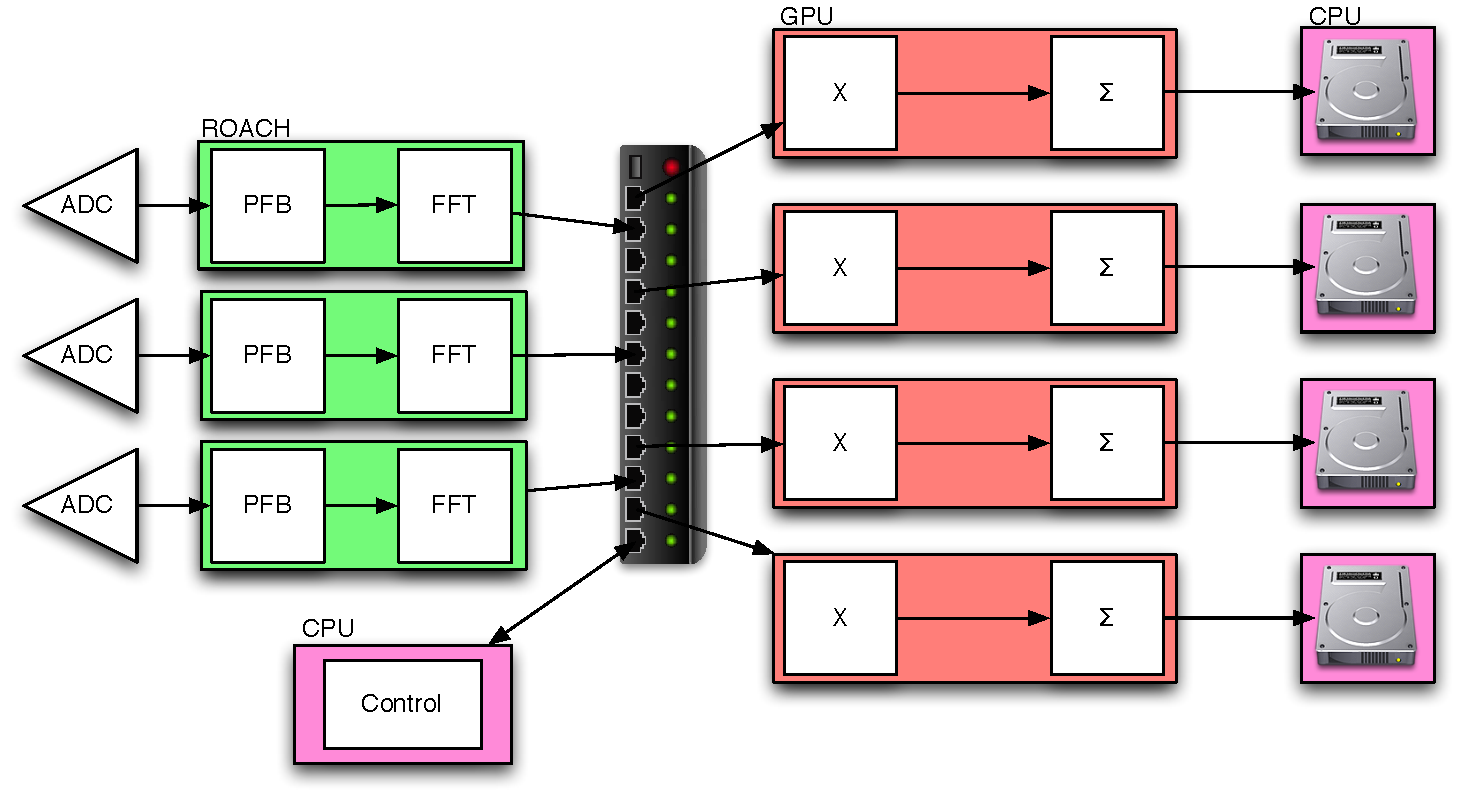
\includegraphics[width=\textwidth]{Images/C4/fx_mapped.pdf}
    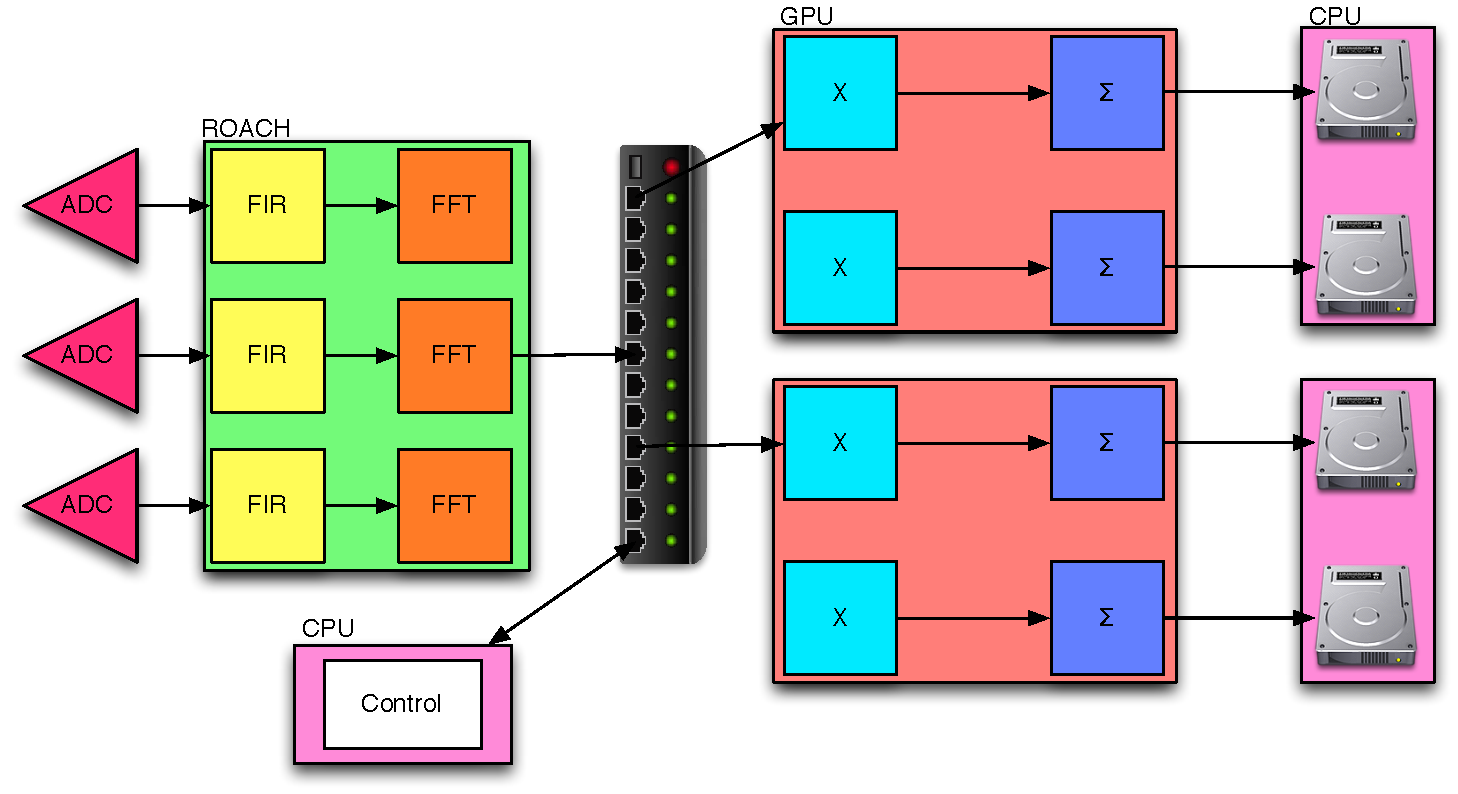
\includegraphics[width=\textwidth]{Images/C4/fx_mapped_alt.pdf}
  \caption{Two potential mappings for the FX Correlator}
  \label{fig: C4/fx_mapped.pdf}
\end{figure}

Once the mapping is complete, the dataflow model is updated to describe what type of hardware will be used to implement each computational block.
Figure \ref{fig: C4/fx_mapped.pdf} shows two or many possible mappings for the FX Correlator dataflow shown in Figure \ref{fig: C4/fx_dataflow.pdf}.
In the top dataflow, each F-engine and X-engine require so many resources that they must be implemented on separate boards.
Each F-engines is implemented on an FPGA-based ROACH board and the X-engines are implemented in GPUs.
The bottom dataflow shows a less resource-hungry correlator, allowing all the F-engines and two X-engines to share a single board for computation.

In all designs, any link between two blocks that are not mapped to the same board must pass through a switch. 
In the example, all the links between FFTs and cross-correlation blocks must run through the switch.
This is represented in the diagram by a single connection from each ROACH and GPU board to the switch.


\section{Code Generation} \label{High Level Toolflow:Code Generation}
The last step in the process is the implementation the instrument. 
This step is optional, only being used when the mapped dataflow is being used to design an instrument rather than assess cost. 
Since the toolflow relies on established libraries, implementation only consists of stitching together existing routines.

%\begin{figure}[ht!]
%  \centering
%    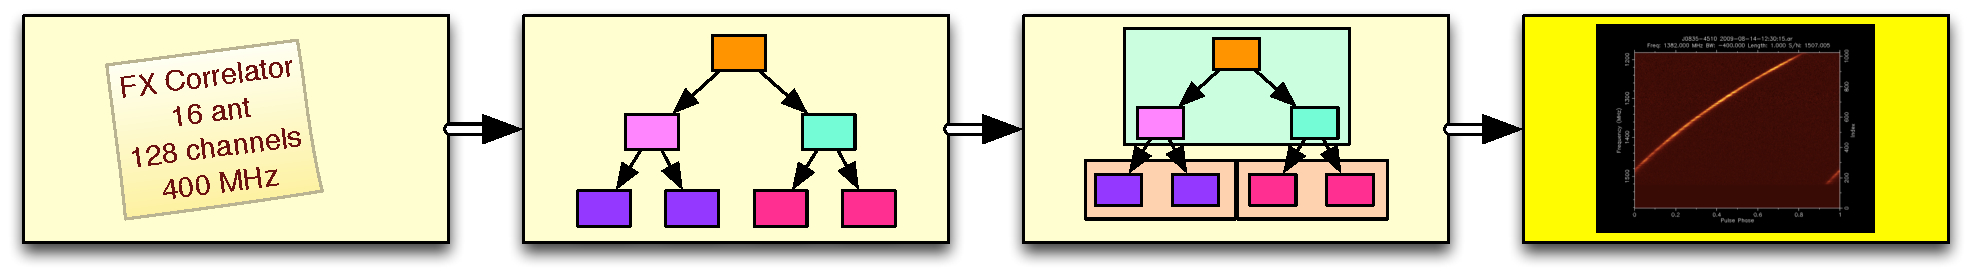
\includegraphics[width=1\textwidth]{Images/C4/toolflow_horizontal_s4.pdf}
%  \caption{The ORCAS Toolflow: Code Generation}
%  \label{fig: C4/toolflow_horizontal_s4.pdf}
%\end{figure}


In addition to this, common design patterns can be stitched together into parameterized implementations. 
This style of instrument design greatly accelerates time to science for many projects.
Separating the implementation of the instrument from the hardware specification has created a design that works well for a variety of computational resources and applications.
As resources improve, the instrument can improve along with them, providing the opportunity to do new science that wasn't possible on older technology.
We have shown this is possible by implementing the Packetized Astronomy Signal Processor or PASP using the CASPER toolflow. \cite{Filiba:2011wl}









